\begin{homeworkProblem}
    
    \textbf{(Coding)} Consider the matrix $A$ and vector $x^*$ defined as
    \begin{equation}
        A = \left[ \begin{array}{ccc} 
            1 & 1 & 1 \\ 
            -1& 1 & 0 \\ 
            -1& -1& 1 \\ 
            1 & 0 & 1 \\ 
            -1& 1 & 1 \\ 
            0 & -1& 1 \end{array}
            \right], \qquad 
        x^* = \left[ \begin{array}{ccc} 
            1 \\ 
            1 \\ 
            1 \end{array}
            \right]
    \end{equation}
 
    Define $b = Ax^* + v$ where $v \in \mathbb R^6$ is some measurement noise. 
    Assume that the user has no access to $x^*$ and aims to learn $x^*$ from 
    the measurement vector $b$. We consider two different estimators to learn 
    $x^*$:
    \begin{subequations}
        \begin{align}
            &\text{$l_1$ estimator:} \qquad \min_x \|Ax-b\|_1, \\
            &\text{$l_2$ estimator:} \qquad \min_x \|Ax-b\|_2
        \end{align}
    \end{subequations}

    Given a solution $\hat x$ obtained from any of the above estimators, we 
    define the estimation error $e = \|\hat x-x^*\|_2$ (note that the error 
    is always computed with respect to the $l_2$-norm no matter which estimator 
    is used for obtaining $\hat x^*$). Assume that the noise $v$ is in the form
    \begin{equation}
        v = \left[ \begin{array}{ccc}  
            t_1 \\ 
            0   \\ 
            0   \\ 
            0   \\ 
            t_2 \\ 
            0   \end{array} \right]
    \end{equation}

    where $t_1$ and $t_2$ are constants that belong to the discrete set 
    $\{-2, -1.9, -1.8, ..., -0.1, 0, 0.1, ..., 1.8, 1.9, 2\}$ (the increment 
    is $0.1$).
    
    \begin{itemize}
        \item [i)] For each possible value of the pair $(t_1, t_2)$, solve the 
            $l_1$ and $l_2$ estimators in CVX and record the corresponding 
            estimation errors (note: there are $41 \times 41$ possibilities 
            for $(t_1, t_2)$). 
        \item [ii)] Draw a grid in $\mathbb R^2$ obtained as follows: For each 
            possible value of the pair $(t_1, t_2)$, we put a symbol in the 
            location $(t_1, t_2)$ in $\mathbb R^2$, where the symbol is a small 
            red circle if the $l_1$ estimator gives the lowest estimation error 
            and is a small blue circle if the $l_2$ estimator gives the lowest 
            estimation error (note: if the estimation errors for both 
            estimators are the same, use the blue circle). Analyze the plot 
            and report your observations. 
    \end{itemize}

    \begin{solution}
        
        I wrote a script in \texttt{problem2.m} to solve the problem
        numerically in CVX. The script iterates through each possible pair
        $(t_1, t_2)$, solves both the $l_1$ and $l_2$ estimators, and
        records the estimation errors. For each pair $(t_1, t_2)$, the 
        script then compares the estimation errors and records which estimator 
        gives the lower error. Finally, the script generates a plot in 
        $\mathbb{R}^2$ indicating which estimator performs better for each 
        possible pair $(t_1, t_2)$, where a small red circle indicates that 
        the $l_1$ estimator gives the lowest estimation error and a small blue 
        circle indicates that the $l_2$ estimator gives the lowest or the same 
        estimation error as that of the $l_1$ estimator.

        \begin{figure}[h!]
            \centering
            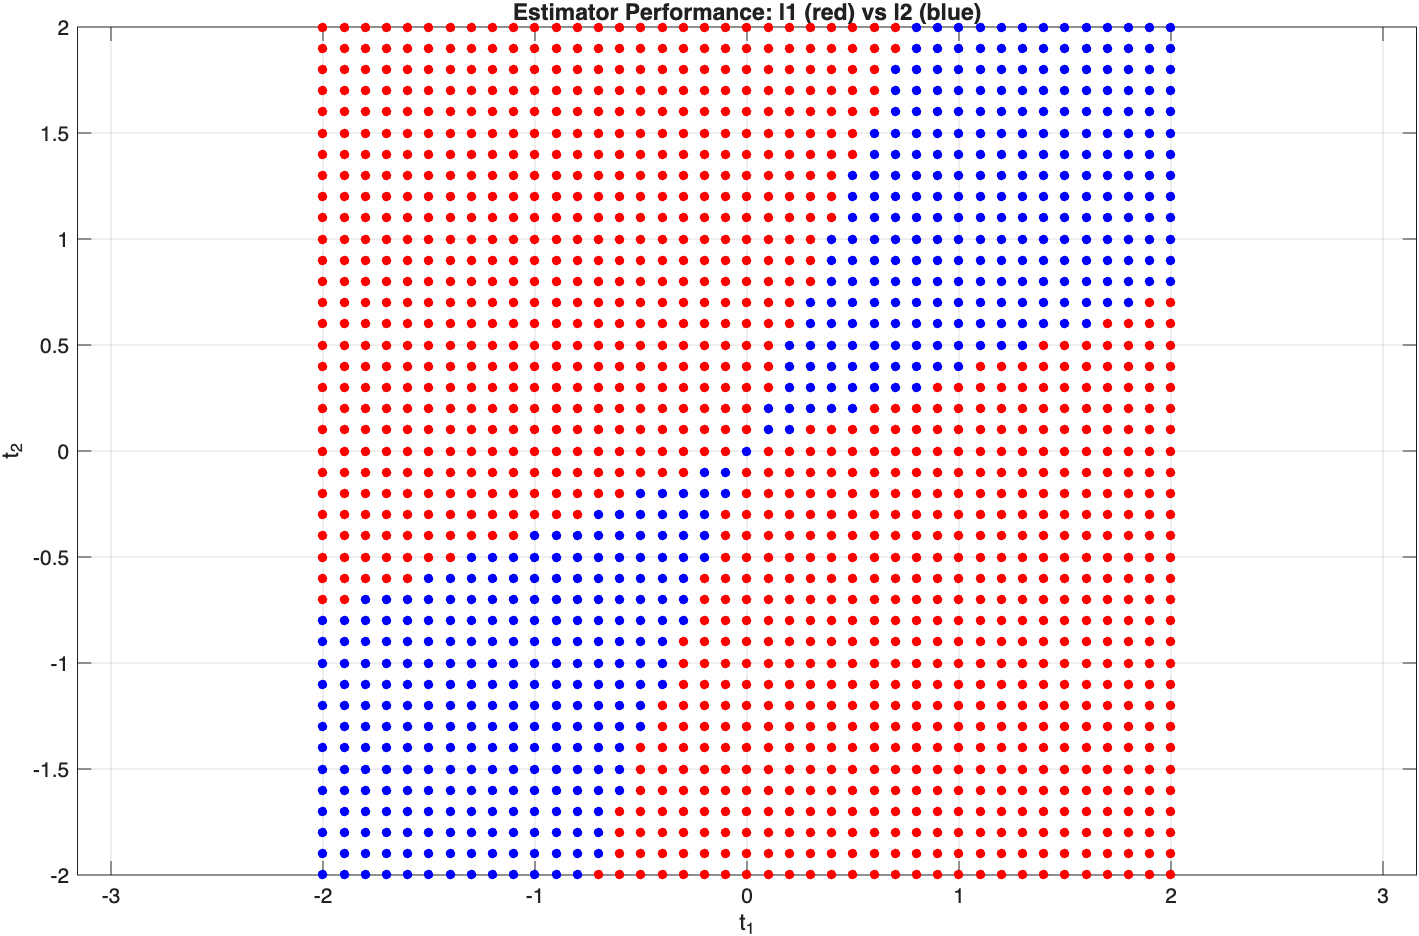
\includegraphics[width=0.75\textwidth]{problem2.png}
        \end{figure}

        \pagebreak

        Above is the plot generated by the script. There is a clear pattern 
        in the performance of the two estimators. The $l_1$ estimator (red 
        circles) performs better in the upper-left quadrant where $t_1$ is
        negative and $t_2$ is positive, and in the lower-right quadrant where 
        $t_1$ is positive and $t_2$ is negative. The $l_2$ estimator 
        (blue circles) dominates in the remaining regions, particularly in 
        the lower-left and upper-right quadrants where $t_1$ and $t_2$ have 
        the same sign, as well as in a thin band in the center, around the
        origin, connecting the two larger regions.
        
        % This suggests that the $l_2$ estimator is more effective when 
        % the noise components have the same sign and sufficient magnitude, 
        % likely due to the $l_2$ norm's robustness to outliers. Conversely, 
        % the $l_2$ estimator performs better when the noise components have 
        % opposite signs or are small in magnitude, which aligns with the 
        % $l_2$ norm's optimality for Gaussian-like noise. The sharp boundaries 
        % between the regions indicate that the relative performance depends 
        % critically on the specific noise structure rather than just the 
        % overall noise magnitude.
            

    \end{solution}

\end{homeworkProblem}